\section{评测 Rubric}

对标 VitaBench 风格的可解释成功率定义，系统内置评测 harness，并设质量门槛（不达标触发重试/降级或人工复核）：

\begin{table}[h]\centering\small
\renewcommand{\arraystretch}{1.2}
\begin{tabularx}{\linewidth}{p{4.6cm} X r}
\toprule
\textbf{指标} & \textbf{含义} & \textbf{结果} \\
\midrule
groundedness & 带有效引用的论断比例 & 1.00 \\
faithfulness & 引用确实支撑论断的比例 & 通过门槛 \\
citation\_hit\_rate & 引用 evidence\_id 逐字命中率 & 1.00 \\
opportunity\_coverage & 提案覆盖的 Top 机会比例 & 0.60 \\
persona\_fidelity & 合成用户来自真实评论 grounding 比例 & 1.00 \\
explainability & 是否产出可解释 DecisionRecord & 1.00 \\
\textbf{overall} & 加权综合 & \textbf{0.875} \\
\bottomrule
\end{tabularx}
\caption{评测 Rubric（样本数据真实运行）}
\end{table}

\section{对比实验：AI 驱动 vs 经验驱动}

命题明确要求"比比看本质不同"。我们将其设计为一个\textbf{受控实验}，而非口头论证：

\begin{itemize}
\item \textbf{同一输入}：相同品类（soundcore TWS 耳机）、相同 brief。
\item \textbf{A 组（经验驱动）}：模拟传统 PM 一次性"拍脑袋"，凭行业常识押注维度，不接数据管线、不做用户验证。
\item \textbf{B 组（AI 原生）}：本系统全链路。
\item \textbf{公平性}：A 组产出的概念也用\textbf{同一份真实数据}评估其"实际会达到的 NPS"，避免只比口号。
\end{itemize}

\begin{table}[h]\centering\small
\renewcommand{\arraystretch}{1.25}
\begin{tabularx}{\linewidth}{X r r r}
\toprule
\textbf{维度} & \textbf{A 经验驱动} & \textbf{B AI 原生} & \textbf{$\Delta$} \\
\midrule
机会覆盖率 & 20\% & \textbf{60\%} & +0.40 \\
命中真实痛点率 & 33\% & \textbf{100\%} & +0.67 \\
证据引用数 & 0 & \textbf{56} & +56 \\
已验证假设数（合成用户） & 0 & \textbf{4} & +4 \\
合成用户数 & 0 & \textbf{4} & +4 \\
可行性风险识别 & 0 & \textbf{3} & +3 \\
预测 NPS & $-29$ & \textbf{+1} & +30 \\
\bottomrule
\end{tabularx}
\caption{AI 驱动 vs 经验驱动（同一 brief，真实数据评估）}
\end{table}

\noindent\textbf{本质不同（五点）：}(1) 从主观到\textbf{可溯源}（每条结论带 evidence\_id 并逐字校验）；
(2) 从少量到\textbf{全量}（统计真实评论全景，不被最响的声音带偏）；(3) 从单次到\textbf{可迭代}（工作流闭环，未达 GO 自动回炉）；
(4) 从拍脑袋到\textbf{可量化}（ODI/Impact/NPS）；(5) 从经验到\textbf{系统能力}（方法论可沉淀为 SOP，复制给任意品类与任意人）。

\section{在线 Demo 截图（数据化）}

\begin{center}
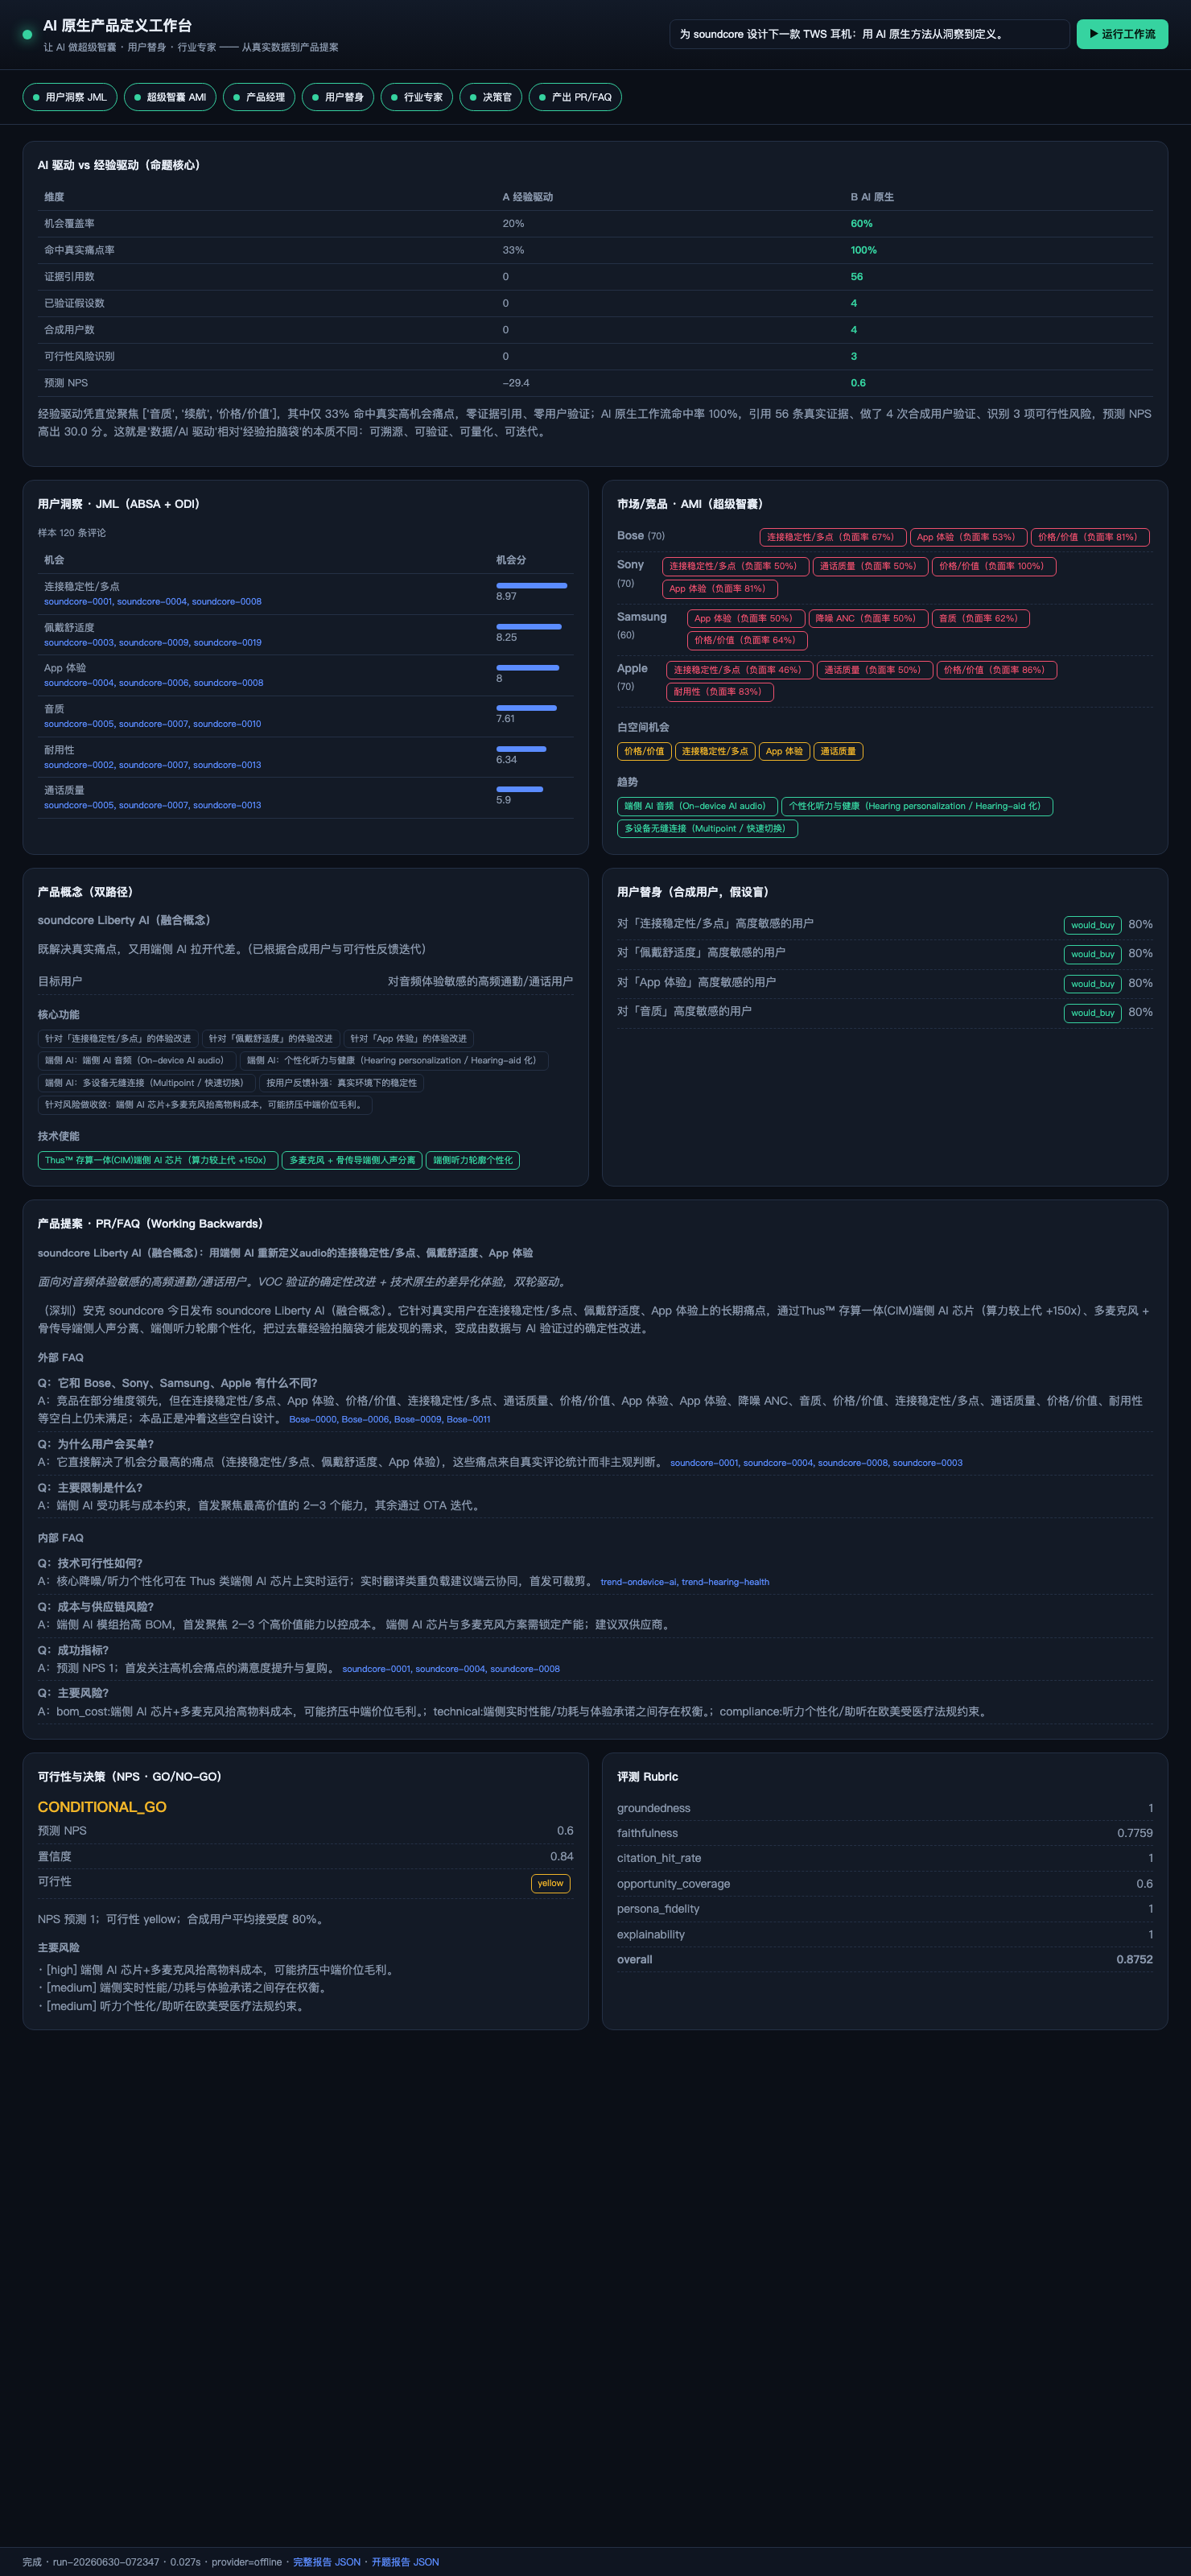
\includegraphics[width=\linewidth]{../figures/demo_full.png}
\captionof{figure}{可视化工作台：每个 Agent 节点实时点亮，并呈现 VOC 机会、竞品白空间、概念、合成用户访谈、PR/FAQ、决策与评测}
\end{center}
